\documentclass[12pt]{article}
\usepackage{multicol}
\usepackage[shortlabels]{enumitem}
\usepackage{tipa}
\usepackage{tikz}
\usetikzlibrary{trees}
\begin{document}
\title{Linguistics 20, Homework 3}
\date{April 22nd, 2019}
\author{Michael Wu\\UID: 404751542\\TA: Eleanor Glewwe\\Discussion 1F Friday 9:00-9:50 AM}
\maketitle

\section*{Chapter 3, Problem 1}

They are separate phonemes, since [p\textsuperscript{h}ul] has a different meaning from [pul]. This is a minimal pair
where the aspirated sound changes the meaning of the word, indicating that they are different.

\section*{Chapter 3, Problem 2}

\paragraph{i)}

The [i] and [u] sounds are different phonemes, since the minimal pair [iglumit] and [iglumut] have different meanings
and only differ by these two sounds. The [a] and [u] sounds are different phonemes, since the minimal pair [anigavit]
and [aniguvit] have different meanings and only differ by these two sounds. The [i] and [a] sounds are different phonemes,
since the minimal pairs [ini] and [ani], [iglu] and [aglu], and [pin\textlengthmark a] and [pan\textlengthmark a] have
different meanings and only differ by these two sounds.

\paragraph{ii)}

[\textsci] is an allophone of the phoneme /i/. [\textupsilon] is an allophone of the phoneme /u/.

\pagebreak

\paragraph{iii)}

\begin{center}
    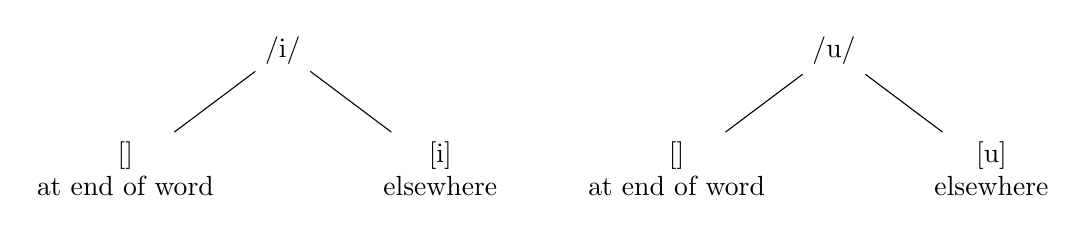
\begin{tikzpicture}[sibling distance = 4cm]
        \node at (-3.5, 0) {/i/} child {node [align=center] {[\textsci]\\at end of word}} child {node [align=center] {[i]\\elsewhere}};
        \node at (3.5, 0) {/u/} child {node [align=center] {[\textupsilon]\\at end of word}} child {node [align=center] {[u]\\elsewhere}};
    \end{tikzpicture}
\end{center}

\paragraph{iv)}

In addition to the features that shared by all vowels, the underlying phoneme of [\textsci] and the underlying phoneme of [\textepsilon] are also
both high and tense. The single feature that distinguishes both [\textsci] from its underlying phoneme and [\textupsilon] from its underlying
phoneme is that [\textsci] and [\textupsilon] are both lax vowels, while their underlying phonemes are tense.

\section*{Chapter 3, Problem 3}

I believe [i] and [\textsubring{i}] are allophones of the same phoneme. Both sounds are high front unrounded tense vowels, but [i]
is voiced while [\textsubring{i}] is unvoiced. In our dataset [i] and [\textsubring{i}] occur in the following mutually exclusive environments.
\begin{center}
    \begin{tabular}{c|c}
        [i] & t\_\#, k\_\#, p\_l, p\_d\\
        \hline
        [\textsubring{i}] & p\_s, k\_s, k\_t
    \end{tabular}
\end{center}
The sound [\textsubring{i}] occurs in locations before a voiceless sound, while [i] occurs elsewhere.
\begin{center}
    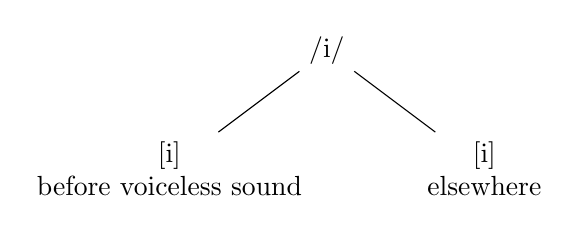
\begin{tikzpicture}[sibling distance = 4cm]
        \node {/i/} child {node [align=center] {[\textsubring{i}]\\before voiceless sound}} child {node [align=center] {[i]\\elsewhere}};
    \end{tikzpicture}
\end{center}

I believe [u] and [\textsubring{u}] are allophones of the same phoneme. Both sounds are high back rounded tense vowels, but [u]
is voiced while [\textsubring{u}] is unvoiced. In our dataset [u] and [\textsubring{u}] occur in the following mutually exclusive environments.
\begin{center}
    \begin{tabular}{c|c}
        [u] & \#\_d, d\_k, l\_d\textyogh, d\textyogh\_k\\
        \hline
        [\textsubring{u}] & t\_p, p\_k, s\_p
    \end{tabular}
\end{center}
The sound [\textsubring{u}] occurs in locations following a voiceless sound, while [u] occurs elsewhere.
\begin{center}
    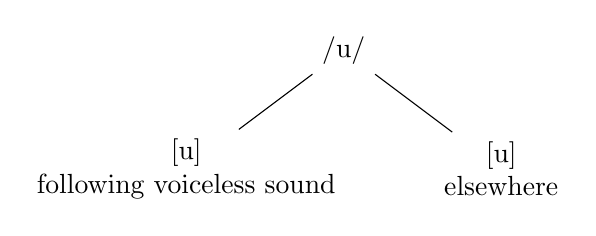
\begin{tikzpicture}[sibling distance = 4cm]
        \node {/u/} child {node [align=center] {[\textsubring{u}]\\following voiceless sound}} child {node [align=center] {[u]\\elsewhere}};
    \end{tikzpicture}
\end{center}

\section*{Chapter 3, Problem 4}

I believe [b] and [\textsubumlaut{b}] are separate phonemes. In our dataset [b] and [\textsubumlaut{b}] occur in the following
environments.
\begin{center}
    \begin{tabular}{c|c}
        [b] & \#\_a, \#\_i, \#\_o\\
        \hline
        [\textsubumlaut{b}] & \#\_a, \#\_i, \#\_\textepsilon, \#\_\textschwa
    \end{tabular}
\end{center}
Although there is no minimal pair, they both occur in the shared environments \#\_a and \#\_i. Thus there is no rule
making them allophones of the same phoneme, so they must be separate phonemes.

\section*{Chapter 3, Problem 5}

I believe [b] and [\textbeta] are allophones of the same phoneme. Both sounds are voiced bilabial consonants, but [b] is a stop while [\textbeta]
is a continuant. In our dataset [b] and [\textbeta] occur in the following mutually exclusive environments.
\begin{center}
    \begin{tabular}{c|c}
        [b] & \#\_r, \#\_a, m\_r, m\_o, \#\_i\\
        \hline
        [\textbeta] & i\_o, o\_i, a\_e, i\_a
    \end{tabular}
\end{center}
The sound [\textbeta] occurs in positions following a vowel while [b] occurs elsewhere.
\begin{center}
    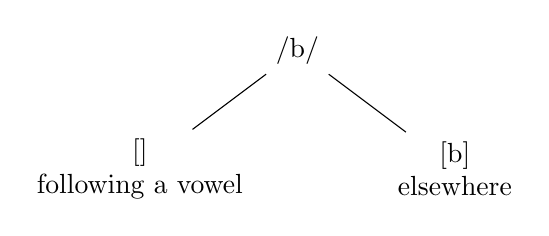
\begin{tikzpicture}[sibling distance = 4cm]
        \node {/b/} child {node [align=center] {[\textbeta]\\following a vowel}} child {node [align=center] {[b]\\elsewhere}};
    \end{tikzpicture}
\end{center}

I believe [d] and [\dh] are allophones of the same phoneme. Both sounds are voiced coronal consonants, but [d] is a stop while [\dh] is a continuant.
In our dataset [d] and [\dh] occur in the following mutually exclusive environments.
\begin{center}
    \begin{tabular}{c|c}
        [d] & \#\_i, \#\_\~u, \#\_u, l\_e, n\_e, u\_z\\
        \hline
        [\dh] & u\_e, y\_\textepsilon, a\_o
    \end{tabular}
\end{center}
The sound [\dh] occurs in positions that are in between vowels while [d] occurs elsewhere.
\begin{center}
    \begin{tikzpicture}[sibling distance = 4cm]
        \node {/d/} child {node [align=center] {[\dh]\\in between vowels}} child {node [align=center] {[d]\\elsewhere}};
    \end{tikzpicture}
\end{center}

I believe [g] and [\textgamma] are allophones of the same phoneme. Both sounds are voiced velar consonants, but [g] is a stop while [\textgamma] is a continuant.
In our dataset [g] and [\textgamma] occur in the following mutually exclusive environments.
\begin{center}
    \begin{tabular}{c|c}
        [g] & \#\_u, \ng\_w, \#\_a, \ng\_\#, a\_r\\
        \hline
        [\textgamma] & i\_a, i\_u, u\_\textepsilon
    \end{tabular}
\end{center}
The sound [\textgamma] occurs in positions that are in between vowels while [g] occurs elsewhere.
\begin{center}
    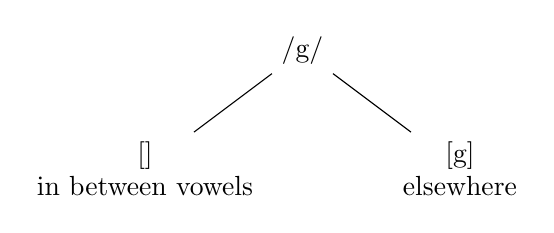
\begin{tikzpicture}[sibling distance = 4cm]
        \node {/g/} child {node [align=center] {[\textgamma]\\in between vowels}} child {node [align=center] {[g]\\elsewhere}};
    \end{tikzpicture}
\end{center}


\section*{Chapter 3, Problem 6}

\paragraph{i)}

I believe [p] and [b] are allophones of the same phoneme. Both sounds are bilabial stopped consonants, but [p] is voiceless while [b] is voiced.
In our dataset [p] and [b] occur in the following mutually exclusive environments.
\begin{center}
    \begin{tabular}{c|c}
        [p] & \#\_a, i\_t, a\_\#, \textschwa\_t, t\_\textschwa\\
        \hline
        [b] & i\_i, a\_\textepsilon, a\_a, \textschwa\_\textschwa, \textepsilon\_u
    \end{tabular}
\end{center}
The sound [b] occurs in positions that are in between vowels while [p] occurs elsewhere.
\begin{center}
    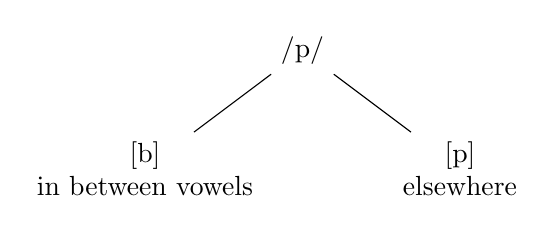
\begin{tikzpicture}[sibling distance = 4cm]
        \node {/p/} child {node [align=center] {[b]\\in between vowels}} child {node [align=center] {[p]\\elsewhere}};
    \end{tikzpicture}
\end{center}

\section*{Chapter 3, Problem 11}

\begin{multicols}{3}
    \begin{enumerate}[a)]
        \item Omitted.
        \item {[continuant]}
        \item {[tense]}
        \item {[high]}
        \item Omitted.
        \item {[anterior]}
        \item {[tense]}
        \item {[voice]}
        \item {[reduced]}
        \item {[strident]}
        \item {[tense]}
        \item {[high]}
    \end{enumerate}
\end{multicols}

\section*{Chapter 3, Problem 12}

\begin{multicols}{2}
    \begin{enumerate}[a)]
        \item \[\left[\begin{tabular}{c}-back\\+tense\end{tabular}\right]\]
        \item \[\left[\begin{tabular}{c}+continuant\\CORONAL\\-anterior\end{tabular}\right]\]
        \item \[\left[\begin{tabular}{c}-round\end{tabular}\right]\]
        \item \[\left[\begin{tabular}{c}+anterior\\-voice\end{tabular}\right]\]
        \item \[\left[\begin{tabular}{c}+voice\end{tabular}\right]\]
        \item \[\left[\begin{tabular}{c}DORSAL\\-back\end{tabular}\right]\]
    \end{enumerate}
\end{multicols}

\end{document}